%%%%%%%%%%%%%%%%%%%%%%%%%%%%%%%%%%%%%%%%%%%%%%%%%%%%%%%%%%%%%%%%%%%%%
% Use the koma-script document style
\documentclass{scrbook}
%\KOMAoptions{twoside=false} % disable two-side formatting for scrbook
% alternatively, for shorter essay, use the following
% \documentclass{scrartcl}
%%%%%%%%%%%%%%%%%%%%%%%%%%%%%%%%%%%%%%%%%%%%%%%%%%%%%%%%%%%%%%%%%%%%%

%%%%%%%%%%%%%%%%%%%%%%%%%%%%%%%%%%%%%%%%%%%%%%%%%%%%%%%%%%%%%%%%%%%%%
% Useful packages
\usepackage{mathtools}
\usepackage{amssymb,bm,bbold}
\usepackage{enumerate}

\usepackage{hhline}
\usepackage{float}

% CSCI-265
\usepackage{tikz}
\usetikzlibrary{automata, positioning, arrows, arrows.meta}


%=================================
% pre-defined theorem environments
\usepackage{amsthm}
\newtheorem{theorem}{Theorem}
\newtheorem{lemma}{Lemma}
\newtheorem{proposition}{Proposition}
\newtheorem{corollary}{Corollary}
\newtheorem{definition}{Definition}
\newtheorem*{remark}{Remark}
\newtheorem*{assumption}{Assumption}

%=================================
% useful commands
\DeclareMathOperator*{\argmin}{arg\,min}
\DeclareMathOperator*{\argmax}{arg\,max}
\DeclareMathOperator*{\supp}{supp}

\def\vec#1{{\ensuremath{\bm{{#1}}}}}
\def\mat#1{\vec{#1}}

%=================================
% convenient notations
\newcommand{\XX}{\mathbb{X}}
\newcommand{\RR}{\mathbb{R}}
\newcommand{\NN}{\mathbb{N}}
\newcommand{\QQ}{\mathbb{Q}}
\newcommand{\ZZ}{\mathbb{Z}}
\newcommand{\EE}{\mathbb{E}}
\newcommand{\PP}{\mathbb{P}}

\newcommand{\sL}{\mathcal{L}}
\newcommand{\sX}{\mathcal{X}}
\newcommand{\sY}{\mathcal{Y}}

\newcommand{\ind}{\mathbb{1}}

\newcommand{\kleene}{{}^\ast}

%%%%%%%%%%%%%%%%%%%%%%%%%%%%%%%%%%%%%%%%%%%%%%%%%%%%%%%%%%%%%%%%%%%%%
% Typography, change document font
\usepackage[tt=false, type1=true]{libertine}
\usepackage[varqu]{zi4}
\usepackage[libertine]{newtxmath}
\usepackage[T1]{fontenc}

\usepackage[protrusion=true,expansion=true]{microtype}

\author{Guy Matz}

\begin{document}
	
\tikzset{
	->, % makes the edges directed 
%		>='stealth', % makes the arrow heads bold 
	node distance=3cm, % specifies the minimum distance between two nodes. Change if necessary. 
	every state/.style={thick, fill=gray!10}, % sets the properties for each ’state’ node 
	initial text=$ $, % sets the text that appears on the start arrow 
}
	
\title{Title}
% \maketitle

% \tableofcontents
% 
% %\bibliography{bibfile}
% 
% \end{document}

	
\begin{enumerate}
	
\item Given the following English descriptions of a language, write a regular expression that defines the language, and draw the state diagram of a DFA that accepts the language. For all languages, let $\Sigma = \{a, b\}$

\begin{enumerate}
	\item The language consisting of all words having a number of a's that is a multiple of 3.
	\\
	Regular Expression: $(a+b)^*(aaa)^*(a+b)^*$
	\\
	State Diagram:\\
	 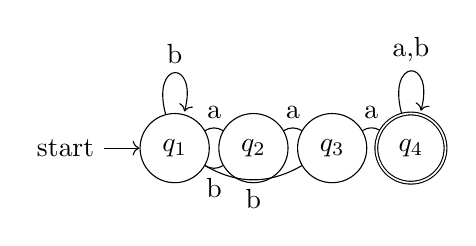
\begin{tikzpicture}
	 	\node[state, initial] (q1) {$q_1$};
	 	\node[state, right of=q1] (q2) {$q_2$};
	 	\node[state, , right of=q2] (q3) {$q_3$};
        \node[state, accepting, right of=q3] (q4) {$q_4$};
	 	\draw
	 	(q1) edge[loop above] node{b} (q1)
	 	(q1) edge[bend  left, above] node{a} (q2)
	  	(q2) edge[bend  left, below] node{b} (q1)
        (q2) edge[bend  left, above] node{a} (q3)
        (q3) edge[bend  left, below] node{b} (q1)
        (q3) edge[bend  left, above] node{a} (q4)
        (q4) edge[loop above] node{a,b} (q4)
	  	;
	 \end{tikzpicture}
	
    \item The language consisting of all words that contain "babb".
    \\
    Regular Expression: $(a+b)^*babb(a+b)^*$
    \\
    State Diagram:\\
    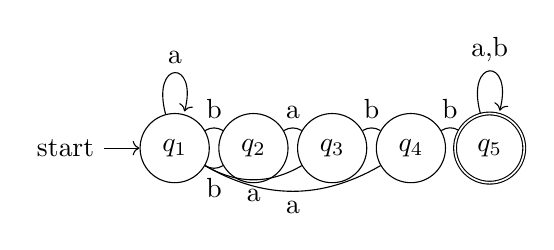
\begin{tikzpicture}
    	\node[state, initial] (q1) {$q_1$};
    	\node[state, right of=q1] (q2) {$q_2$};
    	\node[state, , right of=q2] (q3) {$q_3$};
    	\node[state, , right of=q3] (q4) {$q_4$};
    	\node[state, accepting, right of=q4] (q5) {$q_5$};
    	\draw
    	(q1) edge[loop above] node{a} (q1)
    	(q1) edge[bend  left, above] node{b} (q2)
    	(q2) edge[bend  left, below] node{b} (q1)
    	(q2) edge[bend  left, above] node{a} (q3)
    	(q3) edge[bend  left, below] node{a} (q1)
    	(q3) edge[bend  left, above] node{b} (q4)
    	(q4) edge[bend  left, above] node{b} (q5)
     	(q4) edge[bend  left, below] node{a} (q1)
    	(q5) edge[loop above] node{a,b} (q5)
    	;
    \end{tikzpicture}

    \item The language consisting of all words that end in "ba".
    \\
    Regular Expression: $(a+b)^*ba$
    \\
    State Diagram:\\
    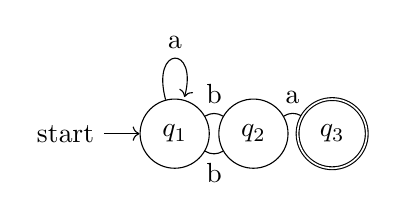
\begin{tikzpicture}
    	\node[state, initial] (q1) {$q_1$};
    	\node[state, right of=q1] (q2) {$q_2$};
    	\node[state, accepting, right of=q2] (q3) {$q_3$};
    	\draw
    	(q1) edge[loop above] node{a} (q1)
    	(q1) edge[bend  left, above] node{b} (q2)
    	(q2) edge[bend  left, below] node{b} (q1)
    	(q2) edge[bend  left, above] node{a} (q3)
    	;
    \end{tikzpicture}

    \item The language consisting of all words that do not end in "ba".
    \\
    Regular Expression: $(a+b)^*(aa + b)$
    \\
    State Diagram:\\
    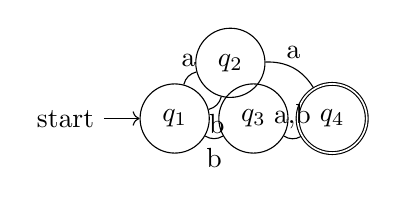
\begin{tikzpicture}
    	\node[state, initial] (q1) {$q_1$};
    	\node[state, above right of=q1] (q2) {$q_2$};
    	\node[state, right of=q1] (q3) {$q_3$};
    	\node[state, accepting, right of=q3] (q4) {$q_4$};
    	\draw
    	(q1) edge[bend  left, above] node{a} (q2)
    	(q2) edge[bend  left, below] node{b} (q1)
    	(q1) edge[bend  right, below] node{b} (q3)
    	(q2) edge[bend  left, above] node{a} (q4)
    	(q3) edge[bend  right, above] node{a,b} (q4)
    	;
    \end{tikzpicture}

\end{enumerate}
\newpage
		
\item John is training for a marathon and he can easily alternate between running a mile and walking a mile. If he runs for 2 miles in a row, he becomes fatigued, and must then walk for 2 miles in a row in order to no longer be fatigued. When he is fatigued, he can still alternate between running a mile and walking a mile, but if he runs 2 miles in a row while already fatigued, he will collapse on the side of the road. If he runs 3 miles in a row at any point, he will also collapse. Let the letter 'a' stand for John running 1 mile, and the letter 'b' stand for John walking 1 mile. Draw a DFA which accepts all possible runs in which John does not collapse on the side of the road.

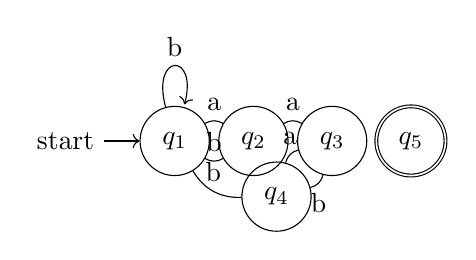
\begin{tikzpicture}
	\node[state, initial] (q1) {$q_1$};
	\node[state, right of=q1] (q2) {$q_2$};
	\node[state, right of=q2] (q3) {$q_3$};
	\node[state, below left of=q3] (q4) {$q_4$};
	\node[state, accepting, right of=q3] (q5) {$q_5$};
	\draw
	(q1) edge[loop above] node{b} (q1)
	(q1) edge[bend  left, above] node{a} (q2)
	(q2) edge[bend  left, above] node{b} (q1)
	(q2) edge[bend  left, above] node{a} (q3)
%	(q3) edge[bend  left, above] node{a} (q5)
	(q3) edge[bend  left, below] node{b} (q4)
	(q4) edge[bend  left, above] node{a} (q3)
	(q4) edge[bend  left, above] node{b} (q1)
	;
\end{tikzpicture}
		
	\newpage
\item Create a DFA to model a vending machine that accepts nickels, dimes, and quarters, and has 2 items for sale, costing 25 cents and 35 cents. Your DFA should take a sequence of inserted coins as input, and accept if you've put in the exact amount for either of the items.
		
\newpage
\item Could we express the language recognized by the DFA in question 3 as a regular expression? How do we know if we could? What would be our approach to writing that regular expression?
		
\newpage
\item What approaches might we take to prove that two regular languages are equivalent? Does it depend on the way in which each language is expressed? List as many ways as you can think of.
		
		
\end{enumerate}

% %\bibliography{bibfile}

\end{document}

